\section{The CERN Accelerator Complex}

CERN (Organisation europeene pour la recherche nucleaire) is a particle physics laboratory near Geneva, Switzerland crossing the Franco-Swiss border between the Swiss commune of Meyrin and French town of Saint-Genis Pouilly. It was founded in 1952 with the creation of the Conseil Europ\'{e}en pour la Recherche Nucl\'{e}aire, which became the Organisation in 1954. It houses an accelerator complex (shown in Fig.~\ref{fig:CERN-acc-complex}) ranging in energies from hundreds of MeV (extraction energy for Linac2) to energies of 7TeV (for the LHC), delivering proton bunches to various experiments (fixed target, colliding and beam) at all energy levels. These experiments have a variety of aims, varying from neutrino physics \cite{Bailey:CNGS}, neutron physics \cite{ntof} antimatter experiments \cite{Gabrielse:ATRAP,Hori:ASACUSA,Hangst:ALPHA} as well as radio isotope \cite{Kadi:ISOLDE} and hadron therapy \cite{Maggiore:ACE} research. The Large Hadron Collider (LHC), the largest accelerator at CERN, is at the forefront of high-energy physics designed to push the energy frontier of knowledge of particle physics.

\begin{figure}
\begin{center}
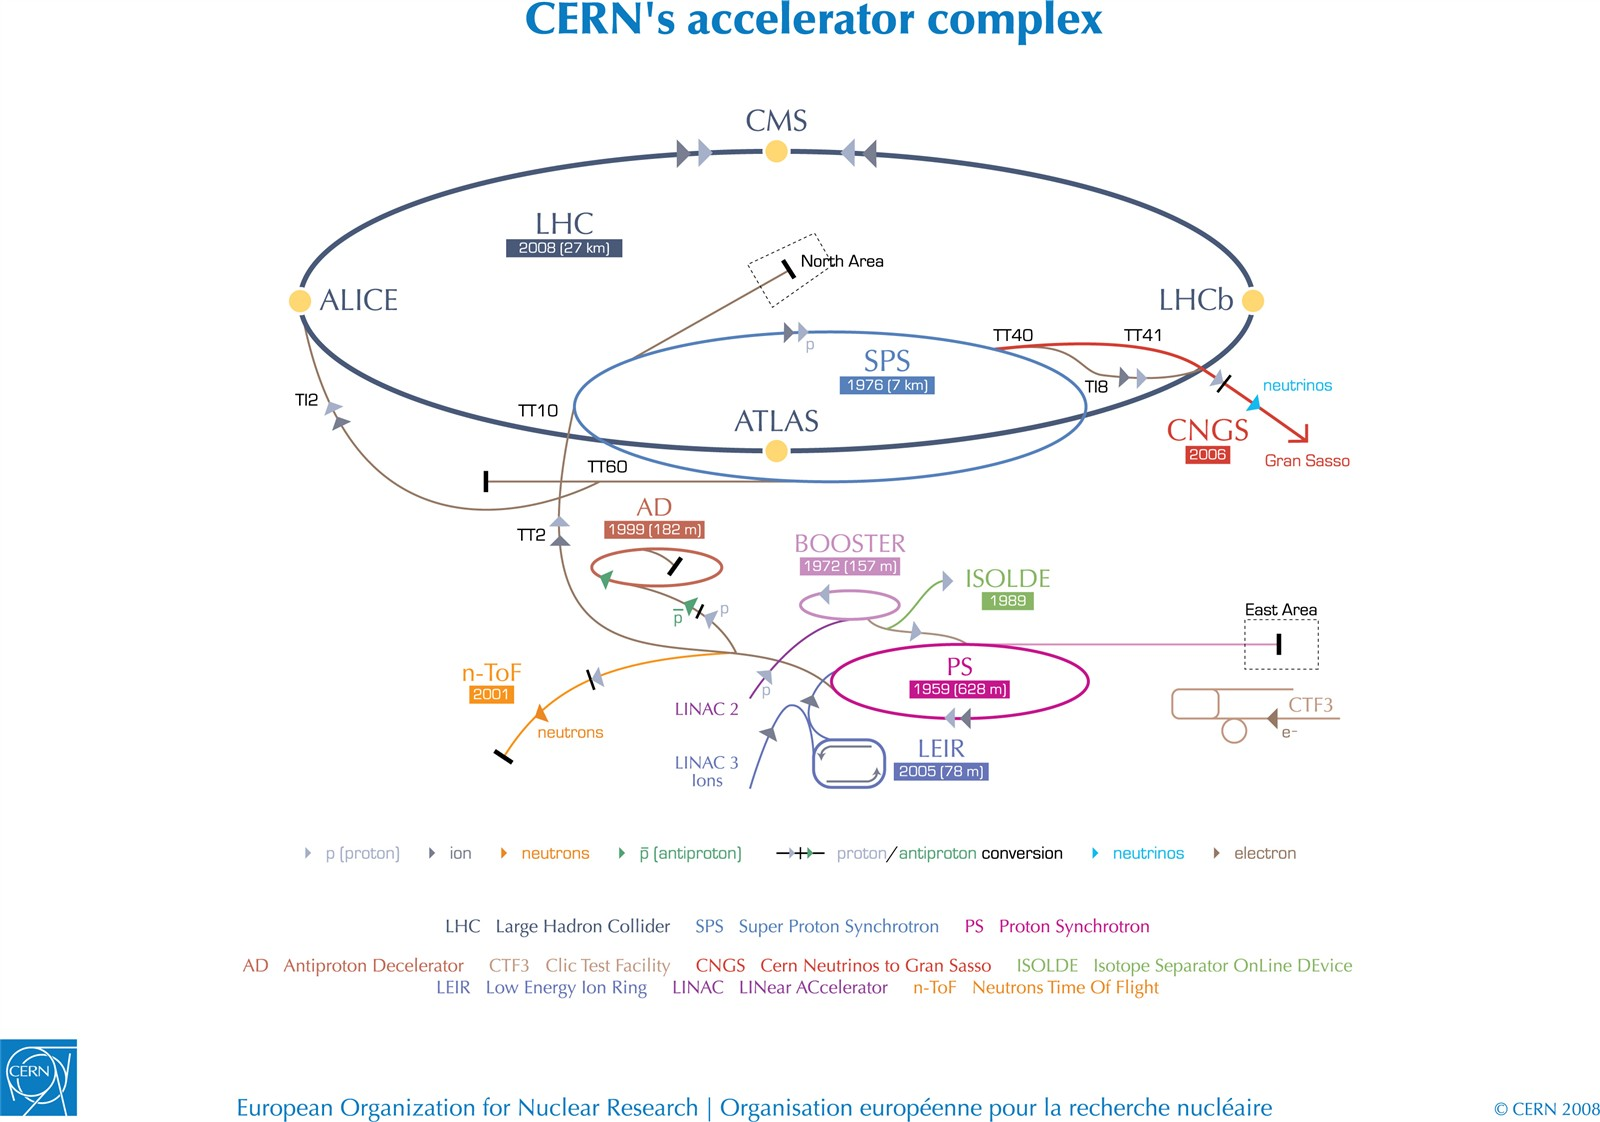
\includegraphics[width=0.95\textwidth]{Introduction/figures/cernaccelerators.jpg}
\end{center}
\label{fig:CERN-acc-complex}
\caption{The CERN accelerator complex, showing both the proton and heavy ion (lead) accelerator chains from LINACs 2 and 3 up to the LHC. Different experimental uses are highlighted in the diagram.}
\end{figure}

\section{The LHC}

The LHC is a synchrotron built to collide counter rotating beams of hadrons at an centre of mass energy of 14TeV for protons and 2.76TeV per nucleon for lead ions. It uses 1,232 superconducting dipole magnets to bend the hadron beams on a circular orbit around the beam line, in addition to using 392 quadrupole magnets for focusing in the transverse plane to maintain the bunch cross section and carry out final focusing for the 4 detector experiments in the LHC. Four detector experments are operated at the LHC; two general purpose detectors ATLAS and CMS, used for searches of new physics beyond the current energy frontier \cite{ATLASTDR,CMSDR}; LHCb, a forward detector specialised in the analysis of B-physics \cite{LHCb} and ALICE, a detector specialised in heavy ion collisions with the intent of observing the physics of quark-gluon plasma \cite{Lourenco:ALICE}. Three further experiments are in place in the LHC, LHCf (an experiment related to the effects of high-energy cosmic rays), TOTEM (measuring the total cross-section of the proton via elastic scattering processes at the collision points) and MoEDAL (an experiment searching for magnetic monopoles and stable massive particles): these three complete the experiments provided with data by collisions using LHC delivered protons.

\section{Operational Figure of Merit - Luminosity}

One of the key figures of merit for the operation of the LHC (along with the centre of mass energy) is the luminosity at the colliding interaction regions (IRs). This is a figure which denotes the total rate of production of new (in the sense of produced during interactions during collisions between protons) particles in collider experiments. It can be thought of as the factor of proportionality between the cross section of a reaction scheme and the number of interactions per second

\begin{equation} 
\frac{dR}{dt} = \mathcal{L} \times \sigma_{p}
\end{equation}

where $\frac{dR}{dt}$ is the interaction rate, $\mathcal{L}$ is the luminosity and $\sigma_{p}$ is the production cross section for a given particle production scheme. For two colliding bunches, each with a gaussian transverse cross-section, the luminosity can be given in a simplified form by

\begin{equation}
\mathcal{L} = \frac{N_{1} N_{2} f n_{b}}{4 \pi \sigma_{x} \sigma_{y}}
\end{equation}

where $N_{1/2}$ is the bunch population of beams 1 and 2 respectively, $f$ is the revolution frequency, $n_{b}$ is the number of colliding bunches in the machine and $\sigma_{x/y}$ is the gaussian bunch sigma in the horizontal and vertical planes respectively. Both the bunch populations $N_{1/2}$, the revoution frequency $f$ and the number of bunches $n_{b}$ also contribute towards the DC beam current in the machine $I_{b} = N_{1} f e n_{b}$ where $e$ is the elementary electron charge. As will be seen in Sec.~\ref{sec:beam_induced_heating} the expected power loss due to beam-equipment interactions is proportional to the $I_{b}^{2}$, thus it can be seen that increasing the luminosity will increase the power loss experienced by equipment in a linear to quadratic fashion (the non-quadratic behaviour being due to other effects on the heating mechanism due to the changing beam current, explained more in Sec.~\ref{sec:beam_induced_heating}).

\subsection{Integrated Luminosity}

Following from the luminosity, the determinant of the quantity of experimental data is the integrated luminosity $\mathcal{L}_{int}$ is given by

\begin{equation}
\mathcal{L}_{int} = \int^{T}_{0} \mathcal{L} \left( t \right) dt
\end{equation}

where $T$ is the integrated collision time and $\mathcal{L} (t)$ is the time varying luminosity (typically decaying exponentially over the lifetime of any given fill of the collider\cite{McCrory:lumiEvo}), varying due to changing beam conditions and bunch populaton depletion due to collisions and particle losses. The integrated luminosity is significant as the number of a given particle production schema observed by the experiments $n_{event}$ is given by

\begin{equation}
n_{event} = \mathcal{L}_{int} \times \sigma_{p}.
\end{equation}

It can thus be seen that in addition to increasing the luminosity, maximising the available time for collisions is important to maximising data collection. This requires a high level of availability of the machine, minimising failures of key systems and the down time experienced by the machine. In particular, unavoidable waiting periods between fills are to be avoided. As is shown in Chapter~\ref{chap:mki}, long cool down times (on the order of hours, similar in magnitude to the length of the average LHC fill) for equipment that requires a specific maximum temperature to operate correctly are thus unacceptable during ideal operation and should be reduced to a minimum. These and other sources of reduction of the running time and luminosity (due to both beam coupling impedance and other sources of instabilities and interlock trips due to hardware mishaps) must thus be carefully studied and controlled by the technical and operations teams.

\section{Beam Dynamics}

To introduce the terms, dynamics and coordinate systems used in later chapters we shall briefly introduce the basic transverse and longitudinal dynamics present in particle accelerators. This introduction follows the formalism introduced in \cite{Holzer:TransDyn}. First we introduce the coordinate system typically used in the consideration of circular particle accelerators. Typically an ideal orbit is defined for an on momentum particle, denoted by $(\rho, \theta, z)$. In addition a reference frame placed upon the orbit of an ideal on-momentum particle is defined, given by $(x, y, z)$, shown in Fig.~\ref{fig:accel-coord-system}. 

\begin{figure}
\begin{center}
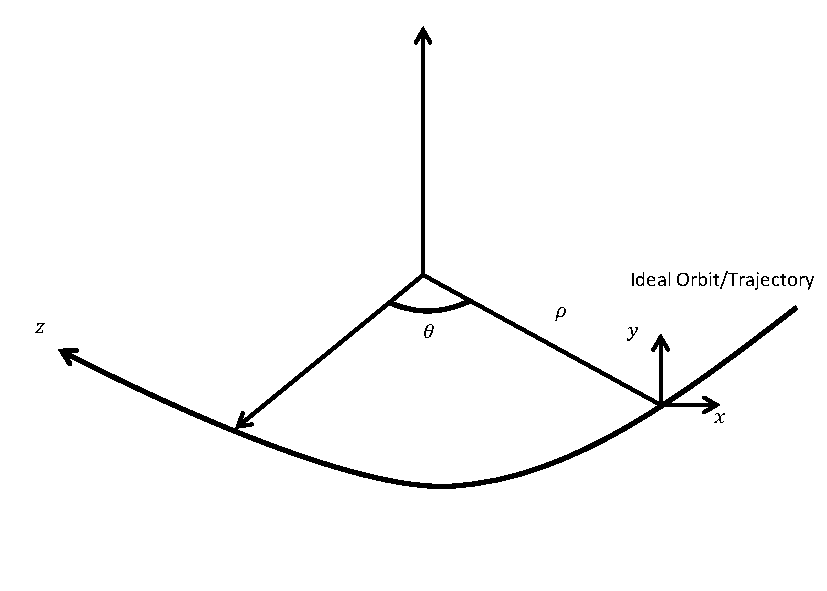
\includegraphics[width=0.75\textwidth]{Introduction/figures/coordinate-system.pdf}
\end{center}
\label{fig:accel-coord-system}
\caption{The representation of the coordinate system of a circular accelerator, and additionally the co-moving reference frame of a circulating particle.}
\end{figure}

\begin{figure}
\begin{center}
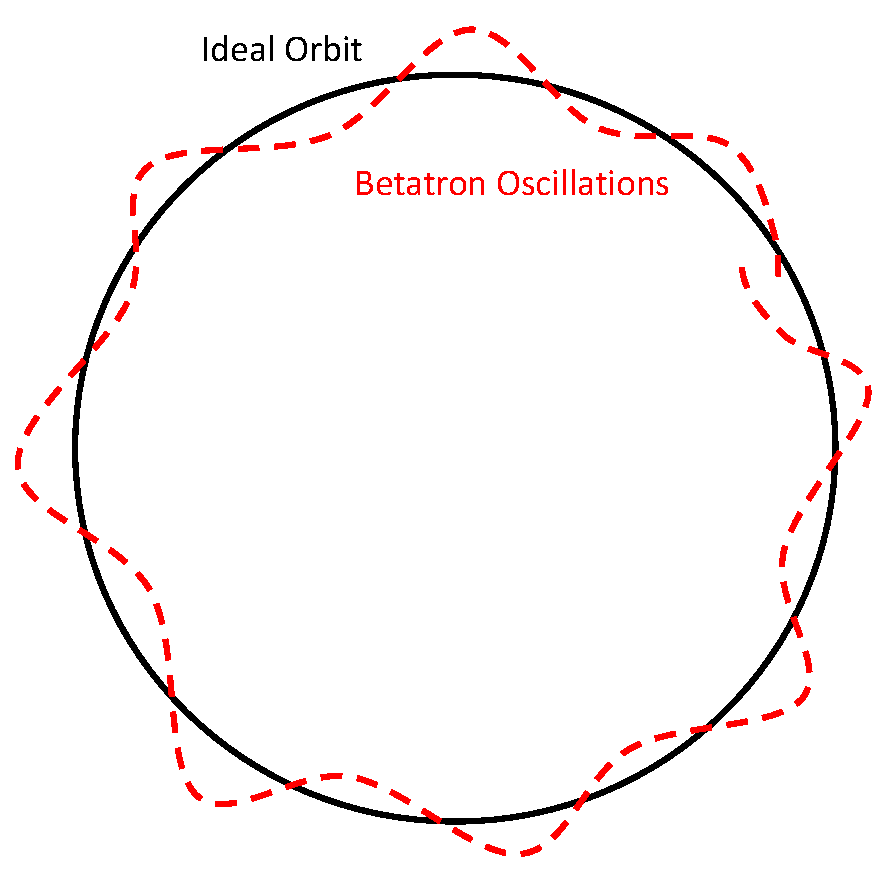
\includegraphics[width=0.65\textwidth]{Introduction/figures/betatron-motion.pdf}
\end{center}
\label{fig:betatron-motion}
\caption{An illustration of betatron oscillations around the ideal orbit of a circular accelerator. These oscillation occur in both the horizontal and vertical planes.}
\end{figure}

The use of charged particles within an accelerator is controlled by the use of both magnetic and electrical elements in the machine, leading to the particles being acted upon by the Lorentz force

\begin{equation}
\mathbf{F} = q \left( \mathbf{E} + \mathbf{v} \times \mathbf{B} \right)
\end{equation}

where $q$ is the charge of the particle, $\mathbf{E}$ is the electric field, $\mathbf{B}$ is the magnetic field and $\mathbf{v}$ is the particles velocity. In high energy particle accelerators the magnetic and electric fields are typically seperated in location, with the magnetic fields only having a transverse component, being of the form

\begin{equation}
\mathbf{B} = \mathbf{\hat{x}} B_{x} + \mathbf{\hat{y}} B_{y}
\end{equation}

where $B_{x/y}$ is the magnetic field component in the $x$- and $y$-axis respectively. Due to the cross product between the velocity ($\mathbf{v} = \mathbf{\hat{z}} v$), it can be seen that there is no component of the force from the magnetic field in the $z$-direction. In addition the electric field usually only has a longitudinal component such that $\mathbf{E} = \mathbf{\hat{z}} E_{z}$. This results in the seperation of transverse and longitudinal motion such that

\begin{align}
F_{\parallel} &= qE \\
\mathbf{F_{\perp}} &= q \left( vB_{y} \mathbf{\hat{x}} - vB_{x} \mathbf{\hat{y}} \right).
\end{align}

Subsequently the transverse and longitudinal motion may both be treated independently of one another.

\subsection{Linear Transverse Dynamics}

If we consider a charged particle of mass $m$ and charge $e$ moving with velocity $v$ along the ideal orbit under the effect of the magnetic field $B$ we can see that the Lorentz force ($F_{L} = qvB$) and the centrifugal force ($F_{cen} = \frac{\gamma m v^{2}}{\rho}$) are equivalent, leading to the relation

\begin{equation}
\frac{p}{e} = B \rho
\label{eqn:beam-rigid}
\end{equation}

where $p$ is the particles momentum. $B \rho$ is referred to as the beam rigidity, denoting the constant term necessary to keep a particle on the ideal orbit. 

If we consider the motion of a particle transversally displaced from the ideal orbit particle with a position $(x, y)$ we must consider the variation of the magnetic field in the transverse directions. If we consider first just the horizontal motion, we can carry out a Taylor expansion of the field which gives us

\begin{equation}
B_{y} \left( x \right) = B_{y0} + \frac{dB_{y}}{dx} x + \frac{1}{2!}\frac{d^{2}B_{y}}{dx^{2}} x^{2} + \frac{1}{3!} \frac{d^{3}B_{y}}{dx^{3}} x^{3} + ...
\end{equation}

which is then normalised by $p/e$

\begin{equation}
\frac{B_{y} \left( x \right)}{p/e} = \frac{B_{y0}}{B_{y0}\rho} + \frac{1}{p/e}\frac{dB_{y}}{dx} x + \frac{1}{p/e}\frac{1}{2!}\frac{d^{2}B_{y}}{dx^{2}} x^{2} + \frac{1}{p/e}\frac{1}{3!} \frac{d^{3}B_{y}}{dx^{3}} x^{3} + ...
\end{equation}

For the time being we shall consider only small displacements in $x$ and $y$, thus shall consider only the linear terms, giving

\begin{align}
\frac{B_{y} \left( x \right)}{p/e} &= \frac{1}{\rho} + \frac{1}{p/e}\frac{dB_{y}}{dx} x \\
\frac{B_{y} \left( x \right)}{p/e} &= \frac{1}{\rho} + k x
\end{align}

where $k = \frac{g}{p/e}$, $g=\frac{2\mu_{0}nI}{r^{2}}$ is the gradient of a quadrupole magnet (a magnet which has a magnetic field strength linearly proportional to displacement), with $n$ being the number of turns on the solenoid, $I$ the current and $r$ the solenoid half-aperture. This indicates that seperation of the function of magnets is valid method of controlling the particles, using dipole and quadrupole fields. Next, to derive the equations of motion we shall consider the equation for radial acceleration $a_{r}$ for a particle undergoing rotational acceleration in the defined coordinate system

\begin{equation}
a_{r} = \frac{d^{2}\rho}{dt^{2}} - \rho \left( \frac{d\theta}{dt} \right)^{2}.
\end{equation}

For the particle on the ideal orbit $\rho = constant$, so $\frac{d \rho}{dt} = 0$, leading to the accelerative force being derived to be

\begin{equation}
F_{x} = m \rho \left( \frac{d\theta}{dt} \right)^{2} = m\rho \omega^{2} = \frac{mv^{2}}{\rho}
\end{equation} 

For a general particle, $\rho \rightarrow \rho + x$, leading to

\begin{equation}
F_{x} = m\frac{d^{2}}{dt^{2}} \left( x+ \rho \right) - \frac{mv^{2}}{x + \rho} = eB_{y} v.
\end{equation}

As $\rho = constant$, $\frac{d^{2}}{dt^{2}} ( x+ \rho )$ becomes $\frac{d^{2}x}{dt^{2}}$. In addition we are dealing with displacements of $x \ll \rho$, so we may approximate $\frac{1}{x+\rho} \approx \frac{1}{\rho}(1-\frac{x}{\rho})$ from the taylor expansion and taking linear terms in $x$. Thus we acquire the equation

\begin{equation}
 m\frac{d^{2}x}{dt^{2}}  - \frac{mv^{2}}{\rho}\left( 1 - \frac{x}{\rho} \right) = eB_{y} v.
\end{equation}

Subsequently we subsitute the magnetic field $B_{y} = B_{y0} + \frac{dB_{y}}{dx} x$ and arrive at

\begin{equation}
 m\frac{d^{2}x}{dt^{2}}  - \frac{mv^{2}}{\rho}\left( 1 - \frac{x}{\rho} \right) = e v \left[ B_{y0} + \frac{dB_{y}}{dx} x \right].
\end{equation}

By dividing throught by the mass m

\begin{equation}
 \frac{d^{2}x}{dt^{2}}  - \frac{v^{2}}{\rho}\left( 1 - \frac{x}{\rho} \right) = \frac{e v B_{y0}}{m} + \frac{ev}{m}\frac{dB_{y}}{dx} x.
\end{equation}

Next we transform the coordinate from $t \rightarrow z$, such that 

\begin{equation}
\frac{d^{2}x}{dt^{2}} = \frac{d}{dt} \left( \frac{dx}{dz} \frac{dz}{dt} \right) = \frac{d}{dz} \left( \frac{dx}{dz} \frac{dz}{dt} \right) \frac{dz}{dt} = \frac{d^{2}x}{dz^{2}}\left( \frac{dz}{dt} \right)^{2} + \frac{dx}{dz} \frac{d}{dz} \left( \frac{dz}{dt} \right) \frac{dz}{dt}.
\end{equation}

It can be seen that $\frac{dz}{dt} = v$, which is kept constant in this treatment. Therefore

\begin{equation}
\frac{d^{2}x}{dt^{2}} = \frac{d^{2}x}{dz^{2}} v^{2}.
\end{equation}

Thus we arrive at the equation

\begin{equation}
\frac{d^{2}x}{dz^{2}} v^{2} - \frac{v^{2}}{\rho}\left( 1 - \frac{x}{\rho} \right) = \frac{e v B_{y0}}{m} + \frac{ev}{m}\frac{dB_{y}}{dx} x.
\end{equation}

We then subsequently normalise by momentum and rearrange slightly to acquire

\begin{equation}
\frac{d^{2}x}{dz^{2}} - \frac{1}{\rho} + \frac{x}{\rho^{2}}  = \frac{ B_{y0}}{p/e} + \frac{1}{p/e}\frac{dB_{y}}{dx} x.
\end{equation}

We then remember the definition of the beam rigidity (see Eqn.~\ref{eqn:beam-rigid}) and the definition of the quadrupolar field strength arriving at

\begin{align}
\frac{d^{2}x}{dz^{2}} - \frac{1}{\rho} + \frac{x}{\rho^{2}}  = - \frac{1}{\rho} + k x \\ \nonumber
\frac{d^{2}x}{dz^{2}} + \frac{x}{\rho^{2}}  = k x \\ \nonumber
\frac{d^{2}x}{dz^{2}} + x \left( \frac{1}{\rho^{2}} - k\right)  = 0.
\label{eqn:horz-eqn-motion}
\end{align}

For the vertical plane the equation is the same, except that the focusing term is negative and there is no $\rho$ term, giving

\begin{equation}
\frac{d^{2}y}{dz^{2}} +  k y  = 0.
\label{eqn:vert-eqn-motion}
\end{equation}

It is interesting to note that there is a focusing term due to the dipolar magnet term. Historically this is the weak focusing effect, as opposed to the strong focusing regime of using quadrupole magnets. It can be seen this these equations are simply the equations of motion of a harmonic oscillator with spring constants $K_{x/y}$ given by

\begin{align*}
K_{x} = \frac{1}{\rho^{2}} - k \\
K_{y} = k
\end{align*}

leading to a general solution 

\begin{equation}
x/y \left( s \right) = a_{1} cos \left( \sqrt{K_{x/y}} s \right) + a_{2} sin \left( \sqrt{K_{x/y}} s \right).
\end{equation}

For a modern particle accelerator using focusing and defocusing magnets arranged in a periodic lattice (i.e. so that $k(s)$ becomes a periodic function such that $k(s+L) = k(s)$ where L is the length of the period of the lattice), and applying initial conditions $x(0) = x_{0}, x^{'}(0) = x^{'}_{0}$ it is possible to finally arrive at the solution for the motion of a particle through a periodic lattice

\begin{equation}
x \left( s \right) = \sqrt{\epsilon} \sqrt{\beta \left( s \right) } cos \left( \psi \left( s \right) + \phi \right)
\end{equation}

where $\epsilon$ and $\phi$ are integration constants determined by the initial conditions, $\beta (s)$ is a periodic function determined by the focusing properties of the lattice. $ \psi (s)$ is the phase advance of the oscillation, again determined by the lattice design parameters. One key important figure acquired from this derivation is the tune (also called the betatron tune) of the accelerator, that is the number of oscillations per turn, given by

\begin{equation}
Q = \frac{1}{2\pi} \oint \frac{ds}{\beta \left( s \right)}.
\end{equation}

\subsubsection{Off-Momentum Particles}

During the operation of a particle accelerator there is often have a spread of particle energies due to dynamics in the longitudinal plane \cite{Leduff:LongDyn}. This gives rise to a momentum spread $\Delta p/p$ in the particle momentum. When considered in Eqn.~\ref{eqn:horz-eqn-motion} this gives rise to an inhomogenous differential equation of the form

\begin{equation}
\frac{d^{2}x}{dz^{2}} + x \left( \frac{1}{\rho^{2}} - k\right)  = \frac{\Delta p}{p}\frac{1}{\rho}
\label{eqn:disp-eqn-motion}
\end{equation}

which leads to a modified solution of the harmonic oscillator equation characterised by the dispersion of the lattice $D(s)$, written as

\begin{equation}
x \left( s \right) = \sqrt{\epsilon} \sqrt{\beta \left( s \right) } cos \left( \psi \left( s \right) + \phi \right) + \frac{\Delta p}{p} D \left( s \right).
\end{equation}

This can be seen as another closed orbit solution to the machine lattice. One side effect of this is the slight change in the tune due to the off momentum particles, characterised by a factor known as the chromaticity $\zeta$, related by

\begin{equation}
\frac{\Delta Q}{Q_{0}} = \zeta \frac{\Delta p}{p}
\end{equation}

where $\Delta Q$ is the tune shift from the lattice tune for an on momentum particle $Q_{0}$. The tune working point is an important factor in designing an accelerator as crossing integer or low order tune fractions (half, third or quarter integer) allows the summation of kicks in the machine driving large oscillations which may ultimately lead to particle loss. 
